%% SECTION HEADER /////////////////////////////////////////////////////////////////////////////////////
\section{Determination of the \acs{madif}}
\label{sec:determination}

%% SECTION CONTENT ////////////////////////////////////////////////////////////////////////////////////
The \ac{madif} is determined based on the function best fitted to indices chosen in the previous subsection.
Since the numerically obtained indices take the shape of a non-linear function, several curves were assumed to find the best fit.
These functions are defined in the general form as follows:
\begin{eqnarray}
	y_1(x,a_i) & = & \frac{a_1x}{x+a_2}+a_3,
	\label{eq:function_1}\\
	y_2(x,a_i) & = & a_1\arctan\left(a_2x\right)+a_3,
	\label{eq:function_2}\\
	y_3(x,a_i) & = & \frac{a_1x}{\sqrt{a_2 + a_3x^2}}+a_4,\label{eq:function_3} 
\end{eqnarray}
where \(a_i\) are the coefficients of the functions.
The coefficients are determined by built-in function of Matlab named \verb+fminsearch+, which searches for the minimum of a problem specified by \(\min\limits_a f(x,a)\), and the function to be optimised is assumed to be \(f(x,a)=\left\|DI_{num} - y(x,a_i)\right\|\), where \(\left\|\cdot\right\|\) means Euclidean norm.
A criterion for evaluating the fit of the curve to simulation results is a mean absolute error defined as the following:
\begin{eqnarray}
	\delta^{\mathrm{fit}} = \sum_{i=1}^{\mathrm{n^{DI}}} \left|\frac{\mathrm{DI^i_{num}}-y(w_d^i)}{\mathrm{DI^i_{num}}}\right|\times\frac{100}{\mathrm{n^{DI}}}\%,
\end{eqnarray}
where \(\mathrm{n^{DI}}\) is the number of index points.
Based on the results from Tab.~\ref{tab:fit_rmsd_full}, \ref{tab:fit_cc_full},  ~\ref{tab:fit_rmsd_homo} and \ref{tab:fit_cc_homo} it turns out that the most fitted function is Eq.~(\ref{eq:function_1}) for most \acp{di}.
The empty cells in the tables mean that the function has been fitted with an error of more than 20\%.
The \ac{di} is no longer taken into account if the fit function has not been established.

\begin{table}
	\small
	\tabcolsep=0.2cm
	\centering
	\caption{\label{tab:fit_rmsd_full} The coefficients and errors of the functions fitted to \acf{rmsd} based on the \acf{fcgm}.}
	\begin{tabular}{ccccccccc}
		\toprule
		\multirow{3}{*}{\rotatebox[origin=c]{90}{Index}} & \multicolumn{2}{c}{Numerical} & \multicolumn{6}{c}{Fit function}\\
		& \multirow{2}{*}{\rotatebox[origin=c]{90}{Model}} & \multirow{2}{*}{\rotatebox[origin=c]{90}{DI\(_{num}\)}} & \multicolumn{2}{c}{Eq.~(\ref{eq:function_1})} & \multicolumn{2}{c}{Eq.~(\ref{eq:function_2})} & \multicolumn{2}{c}{Eq.~(\ref{eq:function_3})}\\
		& & & \(y(w_d^i)\)& \(\delta^{\mathrm{fit}}\) \% & \(y(w_d^i)\) & \(\delta^{\mathrm{fit}}\) \% & \(y(w_d^i)\) & \(\delta^{\mathrm{fit}}\) \%\\
		\midrule
		\multirow{14}{*}{\rotatebox[origin=c]{90}{\ac{rmsd} - 50 \unit{\kHz}}}& \multirow{7}{*}{\rotatebox[origin=c]{90}{\ac{fcgm} - core}}& 1.00 & 1.00 & \multirow{7}{*}{\textcolor{green}{12.73}} & 1.00 & \multirow{7}{*}{14.20} & 1.00 & \multirow{7}{*}{13.95} \\
		& & 0.56 & 0.56 & & 0.61 & & 0.56 & \\
		& & 0.54 & 0.44 & & 0.50 & & 0.41 & \\
		& & 0.53 & 0.40 & & 0.47 & & 0.39 & \\
		& & 0.40 & 0.39 & & 0.46 & & 0.38 & \\
		& & 0.30 & 0.38 & & 0.46 & & 0.38 & \\
		& & 0.44 & 0.37 & & 0.45 & & 0.38 & \\
		\cline{2-9}
		& \multirow{7}{*}{\rotatebox[origin=c]{90}{\ac{fcgm} - interface}}& 1.00 & 1.00 & \multirow{7}{*}{\textcolor{green}{14.35}} & 1.00 & \multirow{7}{*}{16.76} & 1.00 & \multirow{7}{*}{16.11} \\
		& & 0.48 & 0.75 & & 0.82 & & 0.84 & \\
		& & 0.63 & 0.59 & & 0.63 & & 0.63 & \\
		& & 0.48 & 0.53 & & 0.56 & & 0.54 & \\
		& & 0.44 & 0.49 & & 0.53 & & 0.51 & \\
		& & 0.53 & 0.48 & & 0.51 & & 0.49 & \\
		& & 0.48 & 0.46 & & 0.50 & & 0.48 & \\
		\midrule
		\multirow{14}{*}{\rotatebox[origin=c]{90}{\ac{rmsd} - 100 \unit{\kHz}}}& \multirow{7}{*}{\rotatebox[origin=c]{90}{\ac{fcgm} - core}} & 1.00 & 1.00 & \multirow{7}{*}{\textcolor{green}{1.00}} & 1.00 & \multirow{7}{*}{\textcolor{green}{1.00}} & 1.00 & \multirow{7}{*}{1.70} \\
		& & 0.85 & 0.86 & & 0.88 & & 0.85 & \\
		& & 0.78 & 0.78 & & 0.78 & & 0.76 & \\
		& & 0.78 & 0.76 & & 0.75 & & 0.74 & \\
		& & 0.74 & 0.74 & & 0.73 & & 0.74 & \\
		& & 0.72 & 0.73 & & 0.72 & & 0.73 & \\
		& & 0.72 & 0.73 & & 0.72 & & 0.73 & \\
		\cline{2-9}
		& \multirow{7}{*}{\rotatebox[origin=c]{90}{\ac{fcgm} - interface}}& 1.00 & 1.00 & \multirow{7}{*}{\textcolor{green}{1.64}} & 1.00 & \multirow{7}{*}{2.30} & 1.00 & \multirow{7}{*}{2.05} \\
		& & 0.91 & 0.91 & & 0.91 & & 0.92 & \\
		& & 0.84 & 0.81 & & 0.79 & & 0.80 & \\
		& & 0.74 & 0.76 & & 0.73 & & 0.75 & \\
		& & 0.74 & 0.73 & & 0.70 & & 0.73 & \\
		& & 0.69 & 0.71 & & 0.69 & & 0.72 & \\
		& & 0.70 & 0.69 & & 0.68 & & 0.71 & \\
		\bottomrule
	\end{tabular}
\end{table}

\begin{table}
	\small
	\tabcolsep=0.2cm
	\centering
	\caption{\label{tab:fit_cc_full} The coefficients and errors of the functions fitted to \acf{cc} based on the \acf{fcgm}.}
	\begin{tabular}{ccccccccc}
		\toprule
		\multirow{3}{*}{\rotatebox[origin=c]{90}{Index}} & \multicolumn{2}{c}{Numerical} & \multicolumn{6}{c}{Fit function}\\
		& \multirow{2}{*}{\rotatebox[origin=c]{90}{Model}} & \multirow{2}{*}{\rotatebox[origin=c]{90}{DI\(_{num}\)}} & \multicolumn{2}{c}{Eq.~(\ref{eq:function_1})} & \multicolumn{2}{c}{Eq.~(\ref{eq:function_2})} & \multicolumn{2}{c}{Eq.~(\ref{eq:function_3})}\\
		& & & \(y(w_d^i)\)& \(\delta^{\mathrm{fit}}\) \% & \(y(w_d^i)\) & \(\delta^{\mathrm{fit}}\) \% & \(y(w_d^i)\) & \(\delta^{\mathrm{fit}}\) \%\\
		\midrule
		\multirow{14}{*}{\rotatebox[origin=c]{90}{\ac{cc} - 50 \unit{\kHz}}}& \multirow{7}{*}{\rotatebox[origin=c]{90}{\ac{fcgm} - core}}& 1.00 & 1.00 & \multirow{7}{*}{\textcolor{green}{5.49}} & 1.00 & \multirow{7}{*}{6.02} & 1.00 & \multirow{7}{*}{6.18} \\
		& & 0.80 & 0.80 & & 0.79 & & 0.80 & \\
		& & 0.77 & 0.66 & & 0.62 & & 0.62 & \\
		& & 0.68 & 0.60 & & 0.57 & & 0.57 & \\
		& & 0.53 & 0.58 & & 0.55 & & 0.56 & \\
		& & 0.53 & 0.56 & & 0.53 & & 0.55 & \\
		& & 0.54 & 0.54 & & 0.52 & & 0.54 & \\
		\cline{2-9}
		& \multirow{7}{*}{\rotatebox[origin=c]{90}{\ac{fcgm} - interface}}& 1.00 & 1.00 & \multirow{7}{*}{\textcolor{green}{4.21}} & 1.00 & \multirow{7}{*}{\textcolor{green}{4.21}} & 1.00 & \multirow{7}{*}{4.23} \\
		& & 0.82 & 0.82 & & 0.82 & & 0.82 & \\
		& & 0.87 & 0.75 & & 0.75 & & 0.73 & \\
		& & 0.72 & 0.73 & & 0.73 & & 0.72 & \\
		& & 0.67 & 0.72 & & 0.72 & & 0.72 & \\
		& & 0.77 & 0.72 & & 0.72 & & 0.71 & \\
		& & 0.71 & 0.71 & & 0.71 & & 0.71 & \\
		\midrule
		\multirow{14}{*}{\rotatebox[origin=c]{90}{\ac{cc} - 100 \unit{\kHz}}}& \multirow{7}{*}{\rotatebox[origin=c]{90}{\ac{fcgm} - core}}& 1.00 & 1.00 & \multirow{7}{*}{0.45} & \multirow{7}{*}{-} & \multirow{7}{*}{-} & 1.00 & \multirow{7}{*}{0.58} \\
		& & 0.98 & 0.99 & & & & 0.98 & \\
		& & 0.96 & 0.97 & & & & 0.95 & \\
		& & 0.96 & 0.95 & & & & 0.94 & \\
		& & 0.94 & 0.94 & & & & 0.94 & \\
		& & 0.93 & 0.94 & & & & 0.93 & \\
		& & 0.93 & 0.93 & & & & 0.93 & \\
		\cline{2-9}
		& \multirow{7}{*}{\rotatebox[origin=c]{90}{\ac{fcgm} - interface}}& 1.00 & 1.00 & \multirow{7}{*}{\textcolor{green}{0.62}} & \multirow{7}{*}{-} & \multirow{7}{*}{-} & \multirow{7}{*}{-} & \multirow{7}{*}{-} \\
		& & 0.99 & 0.99 & & & & &\\
		& & 0.98 & 0.96 & & & & &\\
		& & 0.95 & 0.95 & & & & &\\
		& & 0.94 & 0.93 & & & & &\\
		& & 0.91 & 0.92 & & & & &\\
		& & 0.92 & 0.92 & & & & &\\
		\bottomrule
	\end{tabular}
\end{table}

\begin{table}
	\small
	\tabcolsep=0.2cm
	\centering
	\caption{\label{tab:fit_rmsd_homo} The coefficients and errors of the functions fitted to \acf{rmsd} based on the \acf{hcgm}.}
	\begin{tabular}{ccccccccc}
		\toprule
		\multirow{3}{*}{\rotatebox[origin=c]{90}{Index}} & \multicolumn{2}{c}{Numerical} & \multicolumn{6}{c}{Fit function}\\
		& \multirow{2}{*}{\rotatebox[origin=c]{90}{Model}} & \multirow{2}{*}{\rotatebox[origin=c]{90}{DI\(_{num}\)}} & \multicolumn{2}{c}{Eq.~(\ref{eq:function_1})} & \multicolumn{2}{c}{Eq.~(\ref{eq:function_2})} & \multicolumn{2}{c}{Eq.~(\ref{eq:function_3})}\\
		& & & \(y(w_d^i)\)& \(\delta^{\mathrm{fit}}\) \% & \(y(w_d^i)\) & \(\delta^{\mathrm{fit}}\) \% & \(y(w_d^i)\) & \(\delta^{\mathrm{fit}}\) \%\\
		\midrule
		\multirow{14}{*}{\rotatebox[origin=c]{90}{\ac{rmsd} - 50 kHz}}& \multirow{7}{*}{\rotatebox[origin=c]{90}{\ac{hcgm} - core}}& 1.00 & 1.00 & \multirow{7}{*}{17.37} & 1.00 & \multirow{7}{*}{19.61} & 1.00 & \multirow{7}{*}{18.51}\\ 
		& & 0.47 & 0.48 & & 0.42 & & 0.49 & \\
		& & 0.41 & 0.35 & & 0.31 & & 0.33 & \\
		& & 0.48 & 0.31 & & 0.29 & & 0.31 & \\
		& & 0.20 & 0.30 & & 0.28 & & 0.30 & \\
		& & 0.28 & 0.29 & & 0.28 & & 0.30 & \\
		& & 0.33 & 0.28 & & 0.27 & & 0.30 & \\
		\cline{2-9}
		& \multirow{7}{*}{\rotatebox[origin=c]{90}{\ac{hcgm} - interface}}& 1.00 & \multirow{7}{*}{-} & \multirow{7}{*}{-} & \multirow{7}{*}{-} & \multirow{7}{*}{-} & \multirow{7}{*}{-} & \multirow{7}{*}{-} \\
		& & 0.23 & & & & & & \\
		& & 0.43 & & & & & & \\
		& & 0.30 & & & & & & \\
		& & 0.17 & & & & & & \\
		& & 0.44 & & & & & & \\
		& & 0.41 & & & & & & \\
		\midrule
		\multirow{14}{*}{\rotatebox[origin=c]{90}{\ac{rmsd} - 100 kHz}}& \multirow{7}{*}{\rotatebox[origin=c]{90}{\ac{hcgm} - core}}& 1.00 & 1.00 & \multirow{7}{*}{\textcolor{green}{4.66}} & 1.00 & \multirow{7}{*}{4.74} & 1.00 & \multirow{7}{*}{6.12} \\
		& & 0.56 & 0.56 & & 0.57 & & 0.57 & \\
		& & 0.58 & 0.50 & & 0.50 & & 0.48 & \\
		& & 0.57 & 0.49 & & 0.49 & & 0.47 & \\
		& & 0.49 & 0.49 & & 0.49 & & 0.47 & \\
		& & 0.49 & 0.48 & & 0.48 & & 0.47 & \\
		& & 0.47 & 0.48 & & 0.48 & & 0.47 & \\
		\cline{2-9}
		& \multirow{7}{*}{\rotatebox[origin=c]{90}{\ac{hcgm} - interface}}& 1.00 & 1.00 & \multirow{7}{*}{\textcolor{green}{7.74}} & 1.00 & \multirow{7}{*}{9.93} & 1.00 & \multirow{7}{*}{10.28} \\
		& & 0.67 & 0.74 & & 0.67 & & 0.67 & \\
		& & 0.62 & 0.56 & & 0.49 & & 0.47 & \\
		& & 0.53 & 0.49 & & 0.44 & & 0.43 & \\
		& & 0.46 & 0.45 & & 0.41 & & 0.42 & \\
		& & 0.34 & 0.42 & & 0.40 & & 0.41 & \\
		& & 0.41 & 0.41 & & 0.39 & & 0.41 & \\
		\bottomrule
	\end{tabular}
\end{table}

\begin{table}
	\small
	\tabcolsep=0.2cm
	\centering
	\caption{\label{tab:fit_cc_homo} The coefficients and errors of the functions fitted to \acf{cc} based on the \acf{hcgm}.}
\begin{tabular}{ccccccccc}
	\toprule
	\multirow{3}{*}{\rotatebox[origin=c]{90}{Index}} & \multicolumn{2}{c}{Numerical} & \multicolumn{6}{c}{Fit function}\\
	& \multirow{2}{*}{\rotatebox[origin=c]{90}{Model}} & \multirow{2}{*}{\rotatebox[origin=c]{90}{DI\(_{num}\)}} & \multicolumn{2}{c}{Eq.~(\ref{eq:function_1})} & \multicolumn{2}{c}{Eq.~(\ref{eq:function_2})} & \multicolumn{2}{c}{Eq.~(\ref{eq:function_3})}\\
	& & & \(y(w_d^i)\)& \(\delta^{\mathrm{fit}}\) \% & \(y(w_d^i)\) & \(\delta^{\mathrm{fit}}\) \% & \(y(w_d^i)\) & \(\delta^{\mathrm{fit}}\) \%\\
	\midrule
		\multirow{14}{*}{\rotatebox[origin=c]{90}{\ac{cc} - 50 kHz}}& \multirow{7}{*}{\rotatebox[origin=c]{90}{\ac{hcgm} - core}}& 1.00 & 1.00 & \multirow{7}{*}{\textcolor{green}{15.37}} & 1.00 & \multirow{7}{*}{15.68} & 1.00 & \multirow{7}{*}{15.83} \\
		& & 0.76 & 0.76 & & 0.76 & & 0.76 & \\
		& & 0.58 & 0.57 & & 0.54 & & 0.52 & \\
		& & 0.66 & 0.49 & & 0.47 & & 0.44 & \\
		& & 0.34 & 0.44 & & 0.43 & & 0.42 & \\
		& & 0.28 & 0.42 & & 0.41 & & 0.40 & \\
		& & 0.40 & 0.40 & & 0.40 & & 0.40 & \\
		\cline{2-9}
		& \multirow{7}{*}{\rotatebox[origin=c]{90}{\ac{hcgm} - interface}}& 1.00 & \multirow{7}{*}{-} & \multirow{7}{*}{-} & \multirow{7}{*}{-} & \multirow{7}{*}{-} & \multirow{7}{*}{-} & \multirow{7}{*}{-}\\
		& & 0.13 & & & & & & \\
		& & 0.60 & & & & & & \\
		& & 0.42 & & & & & & \\
		& & 0.12 & & & & & & \\
		& & 0.59 & & & & & & \\
		& & 0.68 & & & & & & \\
		\midrule
		\multirow{14}{*}{\rotatebox[origin=c]{90}{\ac{cc} - 100 kHz}}& \multirow{7}{*}{\rotatebox[origin=c]{90}{\ac{hcgm} - core}}& 1.00 & 1.00 & \multirow{7}{*}{\textcolor{green}{1.82}} & 1.00 & \multirow{7}{*}{2.04} & 1.00 & \multirow{7}{*}{2.39} \\
		& & 0.80 & 0.80 & & 0.80 & & 0.80 & \\
		& & 0.76 & 0.72 & & 0.71 & & 0.70 & \\
		& & 0.70 & 0.69 & & 0.69 & & 0.69 & \\
		& & 0.65 & 0.68 & & 0.68 & & 0.68 & \\
		& & 0.68 & 0.68 & & 0.68 & & 0.68 & \\
		& & 0.66 & 0.67 & & 0.67 & & 0.68 & \\
		\cline{2-9}
		& \multirow{7}{*}{\rotatebox[origin=c]{90}{\ac{hcgm} - interface}}& 1.00 & 1.00 & \multirow{7}{*}{\textcolor{green}{4.43}} & 1.00 & \multirow{7}{*}{5.07} & 1.00 & \multirow{7}{*}{5.25} \\
		& & 0.84 & 0.89 & & 0.83 & & 0.84 & \\
		& & 0.76 & 0.75 & & 0.67 & & 0.66 & \\
		& & 0.70 & 0.66 & & 0.61 & & 0.60 & \\
		& & 0.58 & 0.59 & & 0.58 & & 0.58 & \\
		& & 0.52 & 0.54 & & 0.57 & & 0.57 & \\
		& & 0.56 & 0.51 & & 0.55 & & 0.56 & \\
		\bottomrule
	\end{tabular}
\end{table}

\begin{figure}
	\begin{center}
		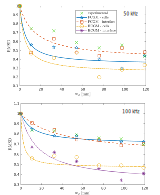
\includegraphics[width=0.95\textwidth]{Chapter_7/rmsd_best}
	\end{center}
	\caption{Comparsion of the \acf{madif} based on \acf{rmsd} and the experimental results.}
	\label{fig:madif_rmsd_best}
\end{figure}
\begin{figure}
	\begin{center}
		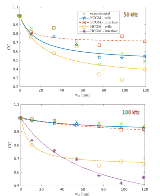
\includegraphics[width=0.95\textwidth]{Chapter_7/cc_best}
	\end{center}
	\caption{Comparsion of the \acf{madif} based on \acf{cc} and the experimental results.}
	\label{fig:madif_cc_best}
\end{figure}
\begin{figure}
	\begin{center}
		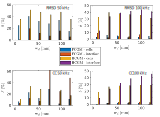
\includegraphics[width=0.95\textwidth]{Chapter_7/MADIF_err}
	\end{center}
	\caption{Percentage absolute error of the \acfp{madif} and the experimental results.}
	\label{fig:madif_err}
\end{figure}

The determined functions and experimental results for the analysed sample are shown in Fig.~\ref{fig:madif_rmsd_best} based on \ac{rmsd} and Fig.~\ref{fig:madif_cc_best} based on \ac{cc}, while the absolute errors between them are in Fig.~\ref{fig:madif_err}.
Both indices of 100 \unit{\kHz} achieved the lowest error for the \ac{fcgm}, with the cells removed as the damage model.
The indices are also in very good agreement for the \ac{fcgm} with removed interface elements as a damage model.
In the case of \ac{hcgm}, unsatisfactory results are not obtained, as none of the indices corresponds to the experimental ones with an error of less than 20\%.
What may be relevant here is that the wave transmits energy to the core throughout its propagation.
In contrast, in the case of \ac{fcgm}, the wave transmits energy incidentally, encountering cell walls.

The comparison of the \ac{madif} and the \ac{edif} based on \ac{rmsd} and \ac{cc} are presented in Fig.~\ref{fig:madif_rmsd} and Fig.~\ref{fig:madif_cc}, respectively.
The \ac{edif} was found using the fit function from Eq.~(\ref{eq:function_1}), the same as the \ac{madif}, for the \acp{di} based on experimental measurements.
In the case of the \ac{rmsd}, the \ac{madif} is in good agreement with the experimental one.
Both functions have a similar trend and aim for a horizontal asymptote of \ac{rmsd}=0.73 and \ac{rmsd}=0.71 for experiments and simulations, respectively.
The absolute error of the damage is no more than 15 \unit{\mm} for damage sizes less than 75 \unit{\mm}.
Above this size, the error increases due to the minimal slope of the function and the different asymptote values.

In the case of the \ac{cc}, the absolute errors are much higher than in the previous index.
As the damage increases, the absolute error increases, as the asymptote values vary considerably.
\begin{figure}[!tbh]
	\begin{center}
		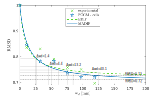
\includegraphics[width=1.0\textwidth]{Chapter_7/MADIF_RMSD}
	\end{center}
	\caption{The \acf{madif} and the \acf{edif} based on the \acf{rmsd} 100 \unit{\kHz}.}
	\label{fig:madif_rmsd}
\end{figure}
\begin{figure}[!tbh]
	\begin{center}
		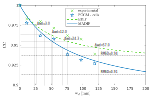
\includegraphics[width=1.0\textwidth]{Chapter_7/MADIF_CC}
	\end{center}
	\caption{The \acf{madif} and the \acf{edif} based on the \acf{cc} 100 \unit{\kHz}.}
	\label{fig:madif_cc}
\end{figure}